\section{\textbf{Hierarchical Backoff Lock}}
\subsection{Particular Case}
\par
The specific case we are trying to solve here is that of mutual exclusion with long waiting times on architectures that make use of hierarchical caching. Let us describe more deeply the characteristics of this scenario.
\par
Firstly, it has already been discussed the difference between \textit{spinning} and \textit{backing-off}. The first case consists on doing an active wait in the case where a $lock()$ operation is not successful. On the other hand, a $backoff$ means that the thread
who failed to acquire the lock refraing from retrying for some duration giving competing threads a chance to finish. As mentioned in the book, the idea is to avoid bus traffic caused by threads asking over and over again for the state of the lock.
\par
The term \textit{Hierarchical} comes from the fact that modern cache-coherent architectures organize processors in clusters. These clusters are organized in such a way that intra-cluster communication is faster than inter-cluster communication. So, the idea in this experiment is to find a lock implementation that takes advantage of these access times differences.
\par
\subsection{Solution}
\par
One of the solutions proposed in the book consists on adapting the \textit{test-and-test-and-set} lock that was described in a previous chapter to exploit the characteristics of the cluster. The idea behind this implementation is that backoff times of local threads should be shorter than backoff times of remote threads. 
\par
\subsection{Experiment Description}
\par
To demonstrate that this implementation works, the test that was provided does the following:
\begin{enumerate}
\item Initiate a shared counter with a value of $0$
\item Start $32$ threads
\item Each thread has to increment the counter by one $32$ times
\item At the end, the counter must hold a value of $32*32$
\end{enumerate}
\par
These are the details of the system we used to run the experiments:
\begin{itemize}
\item Processor: Intel Core i5 @2.5 GHz. 2 Cores.
\item L2 Cache per Core: 256 KB
\item L3 Cache: 3 MB
\item System Memory: 16 GB
\end{itemize}
\subsection{Sample Results}
\par
For this test, we saw that in every try, it always passed.
\par
\begin{figure}[h]
  \centering
  \includegraphics[width=5cm]{HBO00.png}
  \caption{Successful execution of the tests for Hierarchichal Back-off test}
  \label{fig:HBO00}
\end{figure}
\par
\begin{figure}[h]
  \centering
  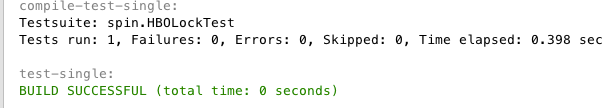
\includegraphics[width=13cm]{HBO01.png}
  \caption{Successful execution of the tests  for Hierarchichal Back-off test}
  \label{fig:HBO01}
\end{figure}
\par
\subsection{Interpretation}
It was shown that the algorithm seems to work and allows synchronization of multiple threads trying to access a shared resource.
\par
One problem however, has to do with the fact that this locking protocol is not fair in the sense that local threads have more chances of acquiring the lock in the next attempt. 
\par
Another thing that we ought to note is that threads spin in the same memory address which causes invalidation of remote cached copies of this value. This problem will be solved yet with another protocol.
